\chapter{Methods}
\label{sec:methods}
%and any classical optimization approaches used for data generation or baseline comparisons.
\section{Numerical implementation}

\section{Convergence tests}
To ensure the numerical stability and accuracy of the RCWA solver, rigorous convergence testing is performed. 
Convergence criteria largely depend on the number of Fourier orders ($N$) retained and the number of layers in the staircase approximation of the fourier patterned grating.
In both cases of figure \ref{fig:convergence_num_layers} and \ref{fig:convergence_order_N}, the error is compared relative to the absorptance curved obtained from the high fidelity comsol simulation of a single fourier patterned grating.

\begin{figure}[htbp]
    \centering
    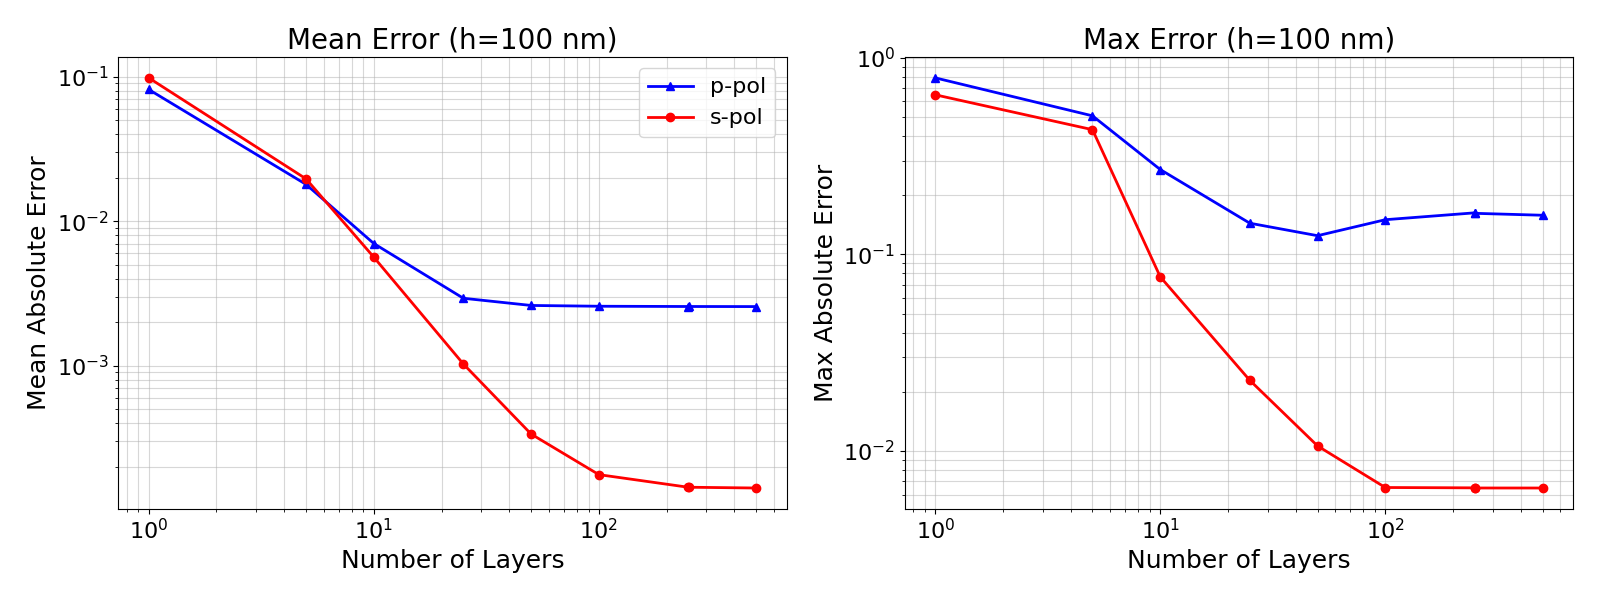
\includegraphics[width=0.85\textwidth]{figures/convergence/convergence_num_layers_100nm.png}
    \caption{Convergence of the RCWA implementation as a function of the number of staircase layers for a grating of height 100 nm.}
    \label{fig:convergence_num_layers}
\end{figure}

\begin{figure}[htbp]
    \centering
    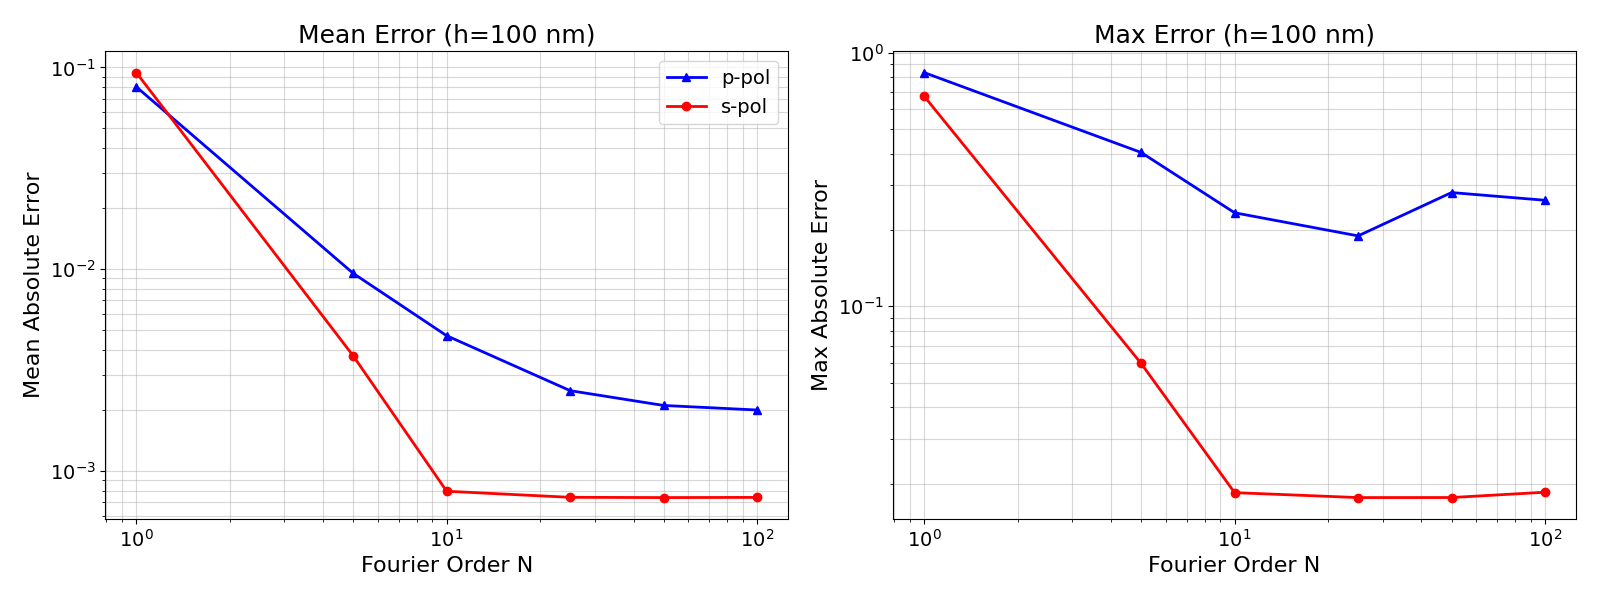
\includegraphics[width=0.85\textwidth]{figures/convergence/convergence_order_N_100nm.png}
    \caption{Convergence of the RCWA implementation as a function of the number of Fourier orders for a grating of height 100 nm.}
    \label{fig:convergence_order_N}
\end{figure}

\begin{figure}[htbp]
    \centering
    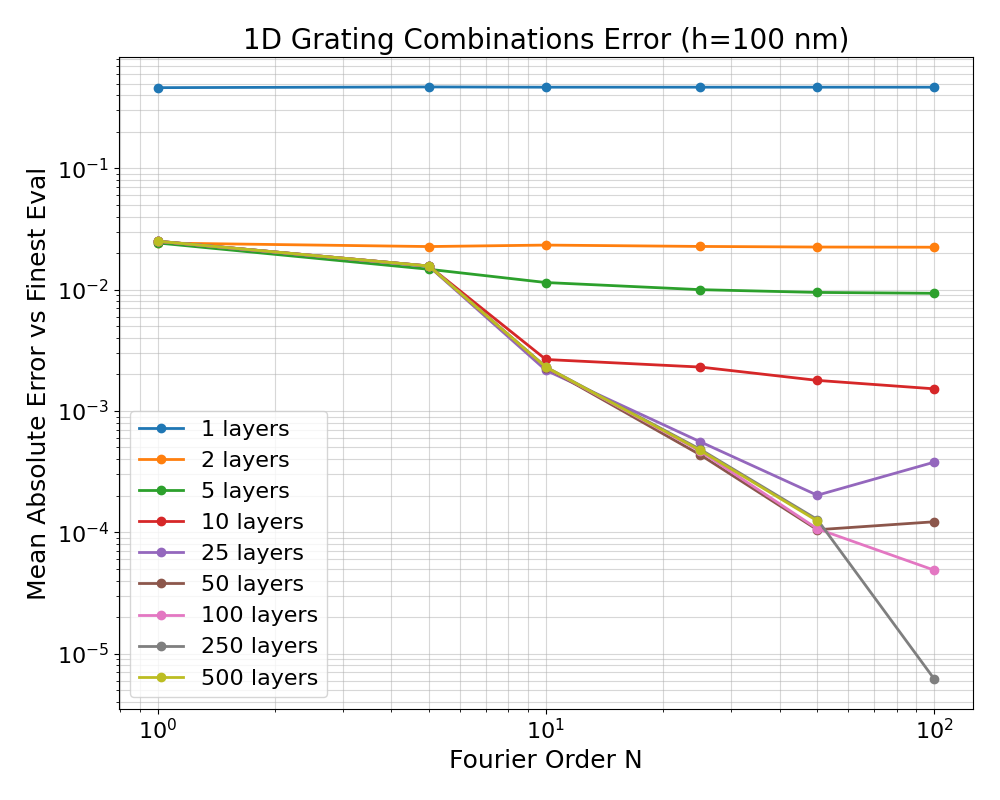
\includegraphics[width=0.48\textwidth]{figures/convergence/sweep_combination_100nm.png}
    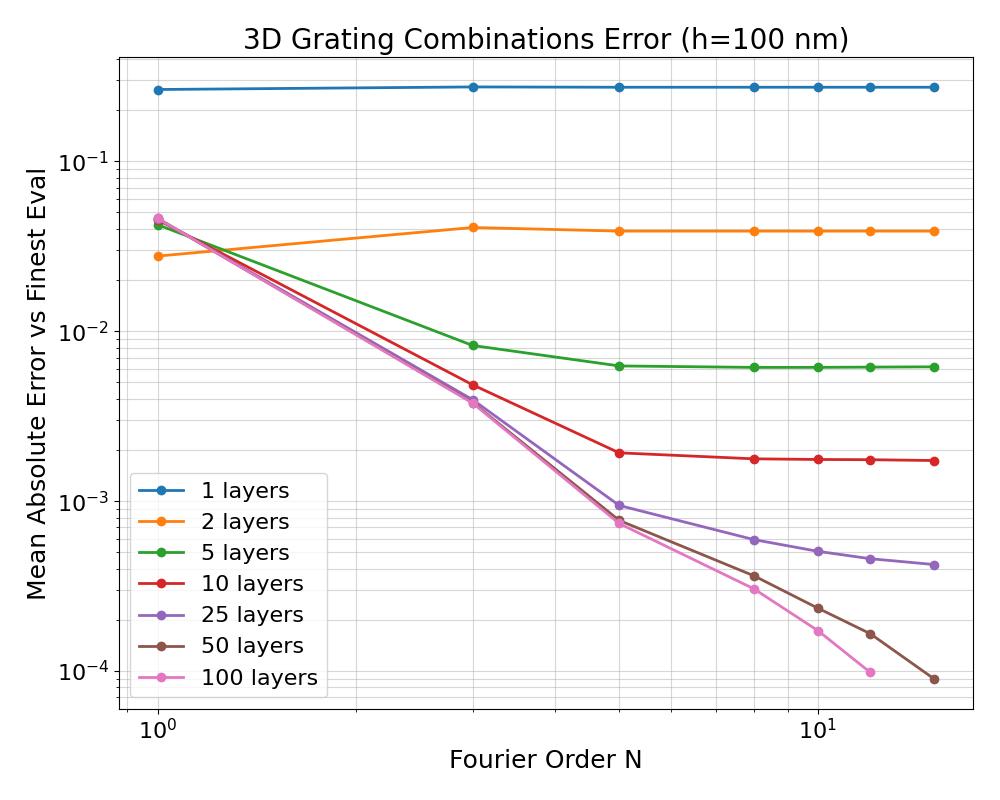
\includegraphics[width=0.48\textwidth]{figures/convergence/sweep_combination_3d_100nm.png}
    \caption{Convergence sweeps and combinations for the 100 nm grating structure. Left: 1D sweep combinations. Right: 3D convergence combinations.}
    \label{fig:convergence_combinations}
\end{figure}

\section{Machine Learning Surrogates}
\label{subsec:ml_surrogates}
% Describe the forward models (e.g., MLP, SpatialCNN, SIREN) and the inverse/generative models (e.g., Tandem networks, Contrastive VAE).

\section{Optimization Strategies}
\label{subsec:optimization_strategies}
% Outline the active learning loop, surrogate optimization techniques, and how candidates are proposed and verified.
